
\section{Preliminaries}
\label{sec:Preliminaries}
In this section, we will present an introduction over the DPLL($\mathcal{T}$) procedure and architecture. The reader can skip this section, if the concepts are clear to them. In the subsequent sections we will present a formal description of the theory solver as a set of normalization rewrite rules, derivation rules and a proof procedure.

\subsection{The DPLL($\mathcal{T}$) Procedure}
\label{sec:dpllt procedure}
In propositional logic, a formula is constructed from a set of boolean variables using a set of logical connectives, such as \(\wedge, \vee, \neg\). Boolean variables can be assigned a truth value that is either  $\texttt{true}$ or  $\texttt{false}$. Given a Boolean formula, the boolean satisfiability problem (SAT) is to answer whether there is an assignment for those variables, such that the formula is evaluated to be $\texttt{true}$. There are many decision procedures to solve the classic SAT problem. Among them, the DPLL procedure is the most frequently used in most modern SAT solvers. 

The DPLL procedure takes a set of clauses as input. It returns $\texttt{sat}$ if a logically consistent assignment can be found; otherwise, it returns $\texttt{unsat}$. During its computation, the procedure maintains an internal stack of literals (possibly with decision marks) to represent a partial assignment. 

Whenever every clause is evaluated to be $\texttt{true}$ under the current assignment, the procedure stops and returns $\texttt{sat}$. During a standard processing loop, the DPLL procedure processes the clause set in three steps:

\begin{description}
	\item[1] It first checks whether the current partial assignment is consistent with the clause set by evaluation. If one of the clauses is evaluated to $\texttt{true}$ and the stack contains at least one decision literal, the procedure pops out all literals in the stack till the nearest decision literal, then flips the sign of that decision literal and turns it into a propagation literal. This step is often referred to \(backtrack\). If one of the clauses is evaluated to $\texttt{false}$ and the stack does not contain one decision literal, the procedure stops and returns $\texttt{unsat}$.
	
	\item[2] After the inconsistent check, the procedure tries to push new propagation literals into the stack by logical deduction. This is known as Unit Propagation.
	
	\item[3] If there are still unassigned variables, the procedure picks one heuristically, guesses its sign, and pushes it into the stack as a decision literal.
\end{description}

The procedure continues until all variables are assigned. In our context, the SAT solver should be able to handle incremental clause assertions. 

\begin{figure}[htb]
	\begin{center}
		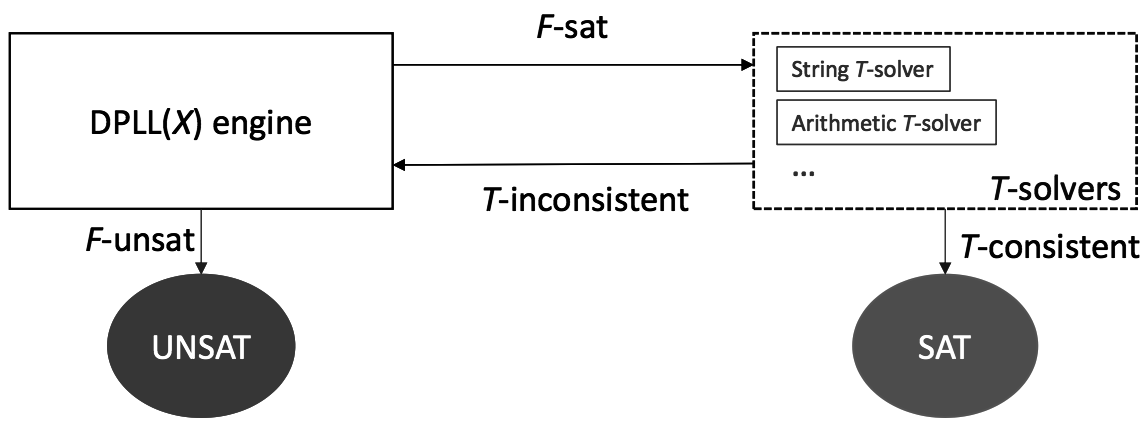
\includegraphics[width=0.8\linewidth]{pictures/dpll_arc.png}
	\end{center}
	\caption{A general DPLL(\(T\)) Architecture. The image is taken from \cite{main_phd}.}
	\label{fig:dpll_architecture}
\end{figure}

\subsection{The DPLL($\mathcal{T}$) Architecture}
\label{sec:The DPLL(T) Architecture}
In Boolean formulas, the signature only contains propositional variables and logical connectives.But in SMT formulas, the signature is extended to a set of predicate symbols, a set of function symbols and a set of non-boolean variables. Those extended symbols can be interpreted in some background theories. An SMT formula is satisfiable if there exists a model that satisfies both the logical formula and the background theories.

Reasoning about an SMT formula usually involves several reasoning over several theories. We refer the procedure to reason over a theory $\mathcal{T}$ as a $\mathcal{T}$-solver. Note that a $\mathcal{T}$-solver can only handle conjunctions of literals. Given a formula over several theories where each theory has a $\mathcal{T}$-solver, the Nelson-Oppen combination \cite{nelson_oppen} provides a procedure to reason about this constraint.

The DPLL($\mathcal{T}$) architecture can be divided into two parts, as shown in Figure \ref{fig:dpll_architecture} : the logic solving part and the theory solving part. In the logic solving part, it usually refers to the DPLL-based SAT solver with  the capability to handle incremental clause assertions. 

The theory solving part usually contains several dedicated solvers for background theories, called $\mathcal{T}$-solvers. Compared to a generic theory solver, a $\mathcal{T}$-solver requires the mechanisms for incrementality and backtracking. A $\mathcal{T}$-solver maintains a set of $\mathcal{T}$-related literals. This set is a subset of the partial assignment $\mathcal{M}$.

Initially, the SAT solver gets the formula $\mathcal{F}$ from the input. It tries to find a model for the literals. If failed, it returns $\texttt{unsat}$; otherwise, it distributes each literal in $\mathcal{M}$ to a corresponding $\mathcal{T}$-solver according to some $\mathcal{T}$-signature-based heuristics.

When a $\mathcal{T}$-solver gets a set of literals, it first checks whether these literals are consistent with the theory. If it is $\mathcal{T}$-consistent, the $\mathcal{T}$-solver does nothing but reports consistent back to the main engine. If it is $\mathcal{M}$-inconsistent, it either returns a conflict (in a form of literal conjunction), or propagates a new literal with an explanation (in a form of implication).

If all $\mathcal{T}$-solvers report $\mathcal{T}$-consistent, the procedure stops and answers $\texttt{sat}$ with the model $\mathcal{M}$; otherwise, the SAT solver collects all clauses returned by $\mathcal{T}$-solvers, and asserts them into the formula $\mathcal{F}$. Then, it tries to build a model from this new formula.

